% Created by tikzDevice version 0.10.1 on 2016-08-23 14:02:44
% !TEX encoding = UTF-8 Unicode
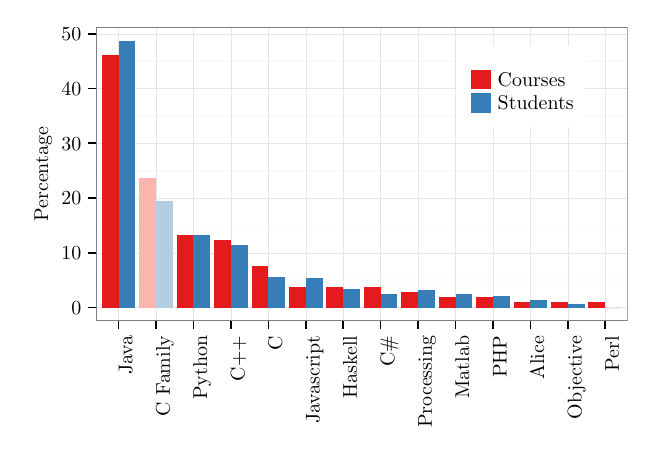
\begin{tikzpicture}[x=1pt,y=1pt]
\definecolor{fillColor}{RGB}{255,255,255}
\path[use as bounding box,fill=fillColor,fill opacity=0.00] (0,0) rectangle (216.81,144.54);
\begin{scope}
\path[clip] (  0.00,  0.00) rectangle (216.81,144.54);
\definecolor{drawColor}{RGB}{255,255,255}
\definecolor{fillColor}{RGB}{255,255,255}

\path[draw=drawColor,line width= 0.6pt,line join=round,line cap=round,fill=fillColor] (  0.00,  0.00) rectangle (216.81,144.54);
\end{scope}
\begin{scope}
\path[clip] ( 24.76, 38.59) rectangle (216.81,144.54);
\definecolor{fillColor}{RGB}{255,255,255}

\path[fill=fillColor] ( 24.76, 38.59) rectangle (216.81,144.54);
\definecolor{drawColor}{gray}{0.98}

\path[draw=drawColor,line width= 0.6pt,line join=round] ( 24.76, 53.30) --
	(216.81, 53.30);

\path[draw=drawColor,line width= 0.6pt,line join=round] ( 24.76, 73.08) --
	(216.81, 73.08);

\path[draw=drawColor,line width= 0.6pt,line join=round] ( 24.76, 92.86) --
	(216.81, 92.86);

\path[draw=drawColor,line width= 0.6pt,line join=round] ( 24.76,112.63) --
	(216.81,112.63);

\path[draw=drawColor,line width= 0.6pt,line join=round] ( 24.76,132.41) --
	(216.81,132.41);
\definecolor{drawColor}{gray}{0.90}

\path[draw=drawColor,line width= 0.2pt,line join=round] ( 24.76, 43.41) --
	(216.81, 43.41);

\path[draw=drawColor,line width= 0.2pt,line join=round] ( 24.76, 63.19) --
	(216.81, 63.19);

\path[draw=drawColor,line width= 0.2pt,line join=round] ( 24.76, 82.97) --
	(216.81, 82.97);

\path[draw=drawColor,line width= 0.2pt,line join=round] ( 24.76,102.75) --
	(216.81,102.75);

\path[draw=drawColor,line width= 0.2pt,line join=round] ( 24.76,122.52) --
	(216.81,122.52);

\path[draw=drawColor,line width= 0.2pt,line join=round] ( 24.76,142.30) --
	(216.81,142.30);

\path[draw=drawColor,line width= 0.2pt,line join=round] ( 32.87, 38.59) --
	( 32.87,144.54);

\path[draw=drawColor,line width= 0.2pt,line join=round] ( 46.40, 38.59) --
	( 46.40,144.54);

\path[draw=drawColor,line width= 0.2pt,line join=round] ( 59.92, 38.59) --
	( 59.92,144.54);

\path[draw=drawColor,line width= 0.2pt,line join=round] ( 73.45, 38.59) --
	( 73.45,144.54);

\path[draw=drawColor,line width= 0.2pt,line join=round] ( 86.97, 38.59) --
	( 86.97,144.54);

\path[draw=drawColor,line width= 0.2pt,line join=round] (100.50, 38.59) --
	(100.50,144.54);

\path[draw=drawColor,line width= 0.2pt,line join=round] (114.02, 38.59) --
	(114.02,144.54);

\path[draw=drawColor,line width= 0.2pt,line join=round] (127.55, 38.59) --
	(127.55,144.54);

\path[draw=drawColor,line width= 0.2pt,line join=round] (141.07, 38.59) --
	(141.07,144.54);

\path[draw=drawColor,line width= 0.2pt,line join=round] (154.60, 38.59) --
	(154.60,144.54);

\path[draw=drawColor,line width= 0.2pt,line join=round] (168.12, 38.59) --
	(168.12,144.54);

\path[draw=drawColor,line width= 0.2pt,line join=round] (181.65, 38.59) --
	(181.65,144.54);

\path[draw=drawColor,line width= 0.2pt,line join=round] (195.17, 38.59) --
	(195.17,144.54);

\path[draw=drawColor,line width= 0.2pt,line join=round] (208.70, 38.59) --
	(208.70,144.54);
\definecolor{fillColor}{RGB}{228,26,28}

\path[fill=fillColor] ( 26.79, 43.41) rectangle ( 32.87,134.84);
\definecolor{fillColor}{RGB}{55,126,184}

\path[fill=fillColor] ( 32.87, 43.41) rectangle ( 38.96,139.72);
\definecolor{fillColor}{RGB}{251,180,174}

\path[fill=fillColor] ( 40.31, 43.41) rectangle ( 46.40, 90.06);
\definecolor{fillColor}{RGB}{179,205,227}

\path[fill=fillColor] ( 46.40, 43.41) rectangle ( 52.48, 81.90);
\definecolor{fillColor}{RGB}{228,26,28}

\path[fill=fillColor] ( 53.84, 43.41) rectangle ( 59.92, 69.53);
\definecolor{fillColor}{RGB}{55,126,184}

\path[fill=fillColor] ( 59.92, 43.41) rectangle ( 66.01, 69.59);
\definecolor{fillColor}{RGB}{228,26,28}

\path[fill=fillColor] ( 67.36, 43.41) rectangle ( 73.45, 67.67);
\definecolor{fillColor}{RGB}{55,126,184}

\path[fill=fillColor] ( 73.45, 43.41) rectangle ( 79.53, 65.87);
\definecolor{fillColor}{RGB}{228,26,28}

\path[fill=fillColor] ( 80.89, 43.41) rectangle ( 86.97, 58.34);
\definecolor{fillColor}{RGB}{55,126,184}

\path[fill=fillColor] ( 86.97, 43.41) rectangle ( 93.06, 54.42);
\definecolor{fillColor}{RGB}{228,26,28}

\path[fill=fillColor] ( 94.41, 43.41) rectangle (100.50, 50.87);
\definecolor{fillColor}{RGB}{55,126,184}

\path[fill=fillColor] (100.50, 43.41) rectangle (106.58, 53.93);
\definecolor{fillColor}{RGB}{228,26,28}

\path[fill=fillColor] (107.93, 43.41) rectangle (114.02, 50.87);
\definecolor{fillColor}{RGB}{55,126,184}

\path[fill=fillColor] (114.02, 43.41) rectangle (120.11, 50.22);
\definecolor{fillColor}{RGB}{228,26,28}

\path[fill=fillColor] (121.46, 43.41) rectangle (127.55, 50.87);
\definecolor{fillColor}{RGB}{55,126,184}

\path[fill=fillColor] (127.55, 43.41) rectangle (133.63, 48.42);
\definecolor{fillColor}{RGB}{228,26,28}

\path[fill=fillColor] (134.98, 43.41) rectangle (141.07, 49.01);
\definecolor{fillColor}{RGB}{55,126,184}

\path[fill=fillColor] (141.07, 43.41) rectangle (147.16, 49.77);
\definecolor{fillColor}{RGB}{228,26,28}

\path[fill=fillColor] (148.51, 43.41) rectangle (154.60, 47.14);
\definecolor{fillColor}{RGB}{55,126,184}

\path[fill=fillColor] (154.60, 43.41) rectangle (160.68, 48.17);
\definecolor{fillColor}{RGB}{228,26,28}

\path[fill=fillColor] (162.03, 43.41) rectangle (168.12, 47.14);
\definecolor{fillColor}{RGB}{55,126,184}

\path[fill=fillColor] (168.12, 43.41) rectangle (174.21, 47.61);
\definecolor{fillColor}{RGB}{228,26,28}

\path[fill=fillColor] (175.56, 43.41) rectangle (181.65, 45.27);
\definecolor{fillColor}{RGB}{55,126,184}

\path[fill=fillColor] (181.65, 43.41) rectangle (187.73, 46.11);
\definecolor{fillColor}{RGB}{228,26,28}

\path[fill=fillColor] (189.08, 43.41) rectangle (195.17, 45.27);
\definecolor{fillColor}{RGB}{55,126,184}

\path[fill=fillColor] (195.17, 43.41) rectangle (201.26, 44.85);
\definecolor{fillColor}{RGB}{228,26,28}

\path[fill=fillColor] (202.61, 43.41) rectangle (208.70, 45.27);
\definecolor{fillColor}{RGB}{55,126,184}

\path[fill=fillColor] (208.70, 43.41) rectangle (214.78, 43.41);
\definecolor{drawColor}{gray}{0.50}

\path[draw=drawColor,line width= 0.6pt,line join=round,line cap=round] ( 24.76, 38.59) rectangle (216.81,144.54);
\end{scope}
\begin{scope}
\path[clip] (  0.00,  0.00) rectangle (216.81,144.54);
\definecolor{drawColor}{RGB}{0,0,0}

\node[text=drawColor,anchor=base east,inner sep=0pt, outer sep=0pt, scale=  0.72] at ( 19.36, 40.93) {0};

\node[text=drawColor,anchor=base east,inner sep=0pt, outer sep=0pt, scale=  0.72] at ( 19.36, 60.71) {10};

\node[text=drawColor,anchor=base east,inner sep=0pt, outer sep=0pt, scale=  0.72] at ( 19.36, 80.49) {20};

\node[text=drawColor,anchor=base east,inner sep=0pt, outer sep=0pt, scale=  0.72] at ( 19.36,100.27) {30};

\node[text=drawColor,anchor=base east,inner sep=0pt, outer sep=0pt, scale=  0.72] at ( 19.36,120.05) {40};

\node[text=drawColor,anchor=base east,inner sep=0pt, outer sep=0pt, scale=  0.72] at ( 19.36,139.82) {50};
\end{scope}
\begin{scope}
\path[clip] (  0.00,  0.00) rectangle (216.81,144.54);
\definecolor{drawColor}{RGB}{0,0,0}

\path[draw=drawColor,line width= 0.6pt,line join=round] ( 21.76, 43.41) --
	( 24.76, 43.41);

\path[draw=drawColor,line width= 0.6pt,line join=round] ( 21.76, 63.19) --
	( 24.76, 63.19);

\path[draw=drawColor,line width= 0.6pt,line join=round] ( 21.76, 82.97) --
	( 24.76, 82.97);

\path[draw=drawColor,line width= 0.6pt,line join=round] ( 21.76,102.75) --
	( 24.76,102.75);

\path[draw=drawColor,line width= 0.6pt,line join=round] ( 21.76,122.52) --
	( 24.76,122.52);

\path[draw=drawColor,line width= 0.6pt,line join=round] ( 21.76,142.30) --
	( 24.76,142.30);
\end{scope}
\begin{scope}
\path[clip] (  0.00,  0.00) rectangle (216.81,144.54);
\definecolor{drawColor}{RGB}{0,0,0}

\path[draw=drawColor,line width= 0.6pt,line join=round] ( 32.87, 35.59) --
	( 32.87, 38.59);

\path[draw=drawColor,line width= 0.6pt,line join=round] ( 46.40, 35.59) --
	( 46.40, 38.59);

\path[draw=drawColor,line width= 0.6pt,line join=round] ( 59.92, 35.59) --
	( 59.92, 38.59);

\path[draw=drawColor,line width= 0.6pt,line join=round] ( 73.45, 35.59) --
	( 73.45, 38.59);

\path[draw=drawColor,line width= 0.6pt,line join=round] ( 86.97, 35.59) --
	( 86.97, 38.59);

\path[draw=drawColor,line width= 0.6pt,line join=round] (100.50, 35.59) --
	(100.50, 38.59);

\path[draw=drawColor,line width= 0.6pt,line join=round] (114.02, 35.59) --
	(114.02, 38.59);

\path[draw=drawColor,line width= 0.6pt,line join=round] (127.55, 35.59) --
	(127.55, 38.59);

\path[draw=drawColor,line width= 0.6pt,line join=round] (141.07, 35.59) --
	(141.07, 38.59);

\path[draw=drawColor,line width= 0.6pt,line join=round] (154.60, 35.59) --
	(154.60, 38.59);

\path[draw=drawColor,line width= 0.6pt,line join=round] (168.12, 35.59) --
	(168.12, 38.59);

\path[draw=drawColor,line width= 0.6pt,line join=round] (181.65, 35.59) --
	(181.65, 38.59);

\path[draw=drawColor,line width= 0.6pt,line join=round] (195.17, 35.59) --
	(195.17, 38.59);

\path[draw=drawColor,line width= 0.6pt,line join=round] (208.70, 35.59) --
	(208.70, 38.59);
\end{scope}
\begin{scope}
\path[clip] (  0.00,  0.00) rectangle (216.81,144.54);
\definecolor{drawColor}{RGB}{0,0,0}

\node[text=drawColor,rotate= 90.00,anchor=base east,inner sep=0pt, outer sep=0pt, scale=  0.72] at ( 37.83, 33.19) {Java};

\node[text=drawColor,rotate= 90.00,anchor=base east,inner sep=0pt, outer sep=0pt, scale=  0.72] at ( 51.36, 33.19) {C Family};

\node[text=drawColor,rotate= 90.00,anchor=base east,inner sep=0pt, outer sep=0pt, scale=  0.72] at ( 64.88, 33.19) {Python};

\node[text=drawColor,rotate= 90.00,anchor=base east,inner sep=0pt, outer sep=0pt, scale=  0.72] at ( 78.41, 33.19) {C++};

\node[text=drawColor,rotate= 90.00,anchor=base east,inner sep=0pt, outer sep=0pt, scale=  0.72] at ( 91.93, 33.19) {C};

\node[text=drawColor,rotate= 90.00,anchor=base east,inner sep=0pt, outer sep=0pt, scale=  0.72] at (105.46, 33.19) {Javascript};

\node[text=drawColor,rotate= 90.00,anchor=base east,inner sep=0pt, outer sep=0pt, scale=  0.72] at (118.98, 33.19) {Haskell};

\node[text=drawColor,rotate= 90.00,anchor=base east,inner sep=0pt, outer sep=0pt, scale=  0.72] at (132.50, 33.19) {C\#};

\node[text=drawColor,rotate= 90.00,anchor=base east,inner sep=0pt, outer sep=0pt, scale=  0.72] at (146.03, 33.19) {Processing};

\node[text=drawColor,rotate= 90.00,anchor=base east,inner sep=0pt, outer sep=0pt, scale=  0.72] at (159.55, 33.19) {Matlab};

\node[text=drawColor,rotate= 90.00,anchor=base east,inner sep=0pt, outer sep=0pt, scale=  0.72] at (173.08, 33.19) {PHP};

\node[text=drawColor,rotate= 90.00,anchor=base east,inner sep=0pt, outer sep=0pt, scale=  0.72] at (186.60, 33.19) {Alice};

\node[text=drawColor,rotate= 90.00,anchor=base east,inner sep=0pt, outer sep=0pt, scale=  0.72] at (200.13, 33.19) {Objective};

\node[text=drawColor,rotate= 90.00,anchor=base east,inner sep=0pt, outer sep=0pt, scale=  0.72] at (213.65, 33.19) {Perl};
\end{scope}
\begin{scope}
\path[clip] (  0.00,  0.00) rectangle (216.81,144.54);
\definecolor{drawColor}{RGB}{0,0,0}

\node[text=drawColor,rotate= 90.00,anchor=base,inner sep=0pt, outer sep=0pt, scale=  0.72] at (  7.36, 91.57) {Percentage};
\end{scope}
\begin{scope}
\path[clip] (  0.00,  0.00) rectangle (216.81,144.54);
\definecolor{fillColor}{RGB}{255,255,255}

\path[fill=fillColor] (155.24,108.74) rectangle (201.56,137.96);
\end{scope}
\begin{scope}
\path[clip] (  0.00,  0.00) rectangle (216.81,144.54);
\definecolor{fillColor}{RGB}{228,26,28}

\path[fill=fillColor] (160.22,122.25) rectangle (167.34,129.37);
\end{scope}
\begin{scope}
\path[clip] (  0.00,  0.00) rectangle (216.81,144.54);
\definecolor{fillColor}{RGB}{55,126,184}

\path[fill=fillColor] (160.22,113.72) rectangle (167.34,120.83);
\end{scope}
\begin{scope}
\path[clip] (  0.00,  0.00) rectangle (216.81,144.54);
\definecolor{drawColor}{RGB}{0,0,0}

\node[text=drawColor,anchor=base west,inner sep=0pt, outer sep=0pt, scale=  0.72] at (169.85,123.33) {Courses};
\end{scope}
\begin{scope}
\path[clip] (  0.00,  0.00) rectangle (216.81,144.54);
\definecolor{drawColor}{RGB}{0,0,0}

\node[text=drawColor,anchor=base west,inner sep=0pt, outer sep=0pt, scale=  0.72] at (169.85,114.80) {Students};
\end{scope}
\end{tikzpicture}
